\documentclass[10pt,a4paper]{article}
\usepackage[utf8]{inputenc}
\usepackage{amsmath}
\usepackage{amsfonts}
\usepackage{amssymb}
\usepackage{amsthm}
\usepackage{float}
\usepackage{mathtools}
\usepackage{geometry}[margin=1in]
\usepackage{xspace}
\usepackage{tikz}
\usepackage{mathrsfs}
\usetikzlibrary{shapes, arrows, decorations.pathmorphing, ducks, automata}
\usepackage[parfill]{parskip}
\usepackage{subcaption}
\usepackage{stmaryrd}
\usepackage{marvosym}
\usepackage{dsfont}
\usepackage{pgfplots}
\usepackage{enumitem}
\usepackage{calc}
\usepackage{tikz-cd}
\usepackage{hyperref}

\hypersetup{
    colorlinks,
    citecolor=black,
    filecolor=black,
    linkcolor=black,
    urlcolor=black
}

\newcommand{\st}{\text{ s.t. }}
\newcommand{\contr}{\lightning}
\newcommand{\im}{\mathfrak{i}}
\newcommand{\R}{\mathbb{R}}
\newcommand{\Q}{\mathbb{Q}}
\newcommand{\C}{\mathbb{C}}
\newcommand{\F}{\mathbb{F}}
\newcommand{\K}{\mathbb{K}}
\newcommand{\N}{\mathbb{N}}
\newcommand{\Z}{\mathbb{Z}}
\renewcommand{\P}{\mathbb{P}}
\renewcommand{\H}{\mathds{H}}
\renewcommand{\O}{\mathcal{O}}
\newcommand{\A}{\mathbb{A}}
\newcommand{\D}{\mathbb{D}}
\newcommand{\nequiv}{\not\equiv}
\newcommand{\powset}{\mathcal{P}}
\renewcommand{\th}[1][th]{\textsuperscript{#1}\xspace}
\newcommand{\from}{\leftarrow}
\newcommand{\legendre}[2]{\left(\frac{#1}{#2}\right)}
\newcommand{\ow}{\text{otherwise}}
\newcommand{\imp}[2]{\underline{\textit{#1.}$\implies$\textit{#2.}}}
\let\oldexists\exists
\let\oldforall\forall
\renewcommand{\exists}{\oldexists\;}
\renewcommand{\forall}{\;\oldforall}
\renewcommand{\hat}{\widehat}
\renewcommand{\tilde}{\widetilde}
\newcommand{\one}{\mathds{1}}
\newcommand{\under}{\backslash}
\newcommand{\injection}{\hookrightarrow}
\newcommand{\surjection}{\twoheadrightarrow}
\newcommand{\jacobi}{\legendre}
\newcommand{\floor}[1]{\lfloor #1 \rfloor}
\newcommand{\ceil}[1]{\lceil #1 \rceil}
\newcommand{\cbrt}[1]{\sqrt[3]{#1}}
\renewcommand{\angle}[1]{\langle #1 \rangle}
\newcommand{\dbangle}[1]{\angle{\angle{#1}}}
\newcommand{\wrt}{\text{ w.r.t. }}

\newcommand*\circled[1]{\tikz[baseline=(char.base)]{
      \node[shape=circle,draw,inner sep=2pt] (char) {#1};}
}

\DeclareMathOperator{\ex}{ex}
\DeclareMathOperator{\id}{id}
\DeclareMathOperator{\upper}{Upper}
\DeclareMathOperator{\dom}{dom}
\DeclareMathOperator{\disc}{disc}
\DeclareMathOperator{\charr}{char}
\DeclareMathOperator{\Image}{im}
\DeclareMathOperator{\ord}{ord}
\DeclareMathOperator{\lcm}{lcm}
\DeclareMathOperator{\aut}{Aut}
\DeclareMathOperator{\diag}{diag}
\DeclareMathOperator{\stab}{stab}
\DeclareMathOperator{\trace}{trace}
\DeclareMathOperator{\ecl}{ecl}
\DeclareMathOperator{\Span}{Span}
\DeclareMathOperator{\Gal}{Gal}
\DeclareMathOperator{\Aut}{Aut}
\DeclareMathOperator{\Frob}{Frob}
\let\div\relax
\DeclareMathOperator{\div}{div}
\DeclareMathOperator{\Div}{Div}
\let\Re\relax
\let\Im\relax
\DeclareMathOperator{\Re}{\mathfrak{Re}}
\DeclareMathOperator{\Im}{\mathfrak{Im}}
\DeclareMathOperator{\Frac}{Frac}
\DeclareMathOperator{\Pic}{Pic}

\let\emph\relax
\DeclareTextFontCommand{\emph}{\bfseries\em}

\newtheorem{theorem}{Theorem}[section]
\newtheorem{lemma}[theorem]{Lemma}
\newtheorem{corollary}[theorem]{Corollary}
\newtheorem{proposition}[theorem]{Proposition}
\newtheorem{conjecture}[theorem]{Conjecture}
\newtheorem{definition}[theorem]{Definition}

\definecolor{burgundy}{rgb}{0.5, 0.0, 0.13}

\tikzset{sketch/.style={decorate,
 decoration={random steps, amplitude=1pt, segment length=5pt},
 line join=round, draw=black!80, very thick, fill=#1
}}


\title{Elliptic Curves}
\begin{document}
\maketitle
\tableofcontents
\newpage
\section{Fermat's Method of Infinite Descent}
Suppose we have a right-angled triangle $\Delta$ with side lengths $a, b, c$, so that by Pythagoras we have $a^2 + b^2 = c^2$, and $\text{area}(\Delta) = \frac12 ab$.
\begin{definition}
  $\Delta$ is \emph{rational} if $a, b, c \in \Q$, and \emph{primitive} if $a, b, c \in \Z$ coprime.
\end{definition}
\begin{lemma}
  Every primitive triangle is of the form $a = u^2-v^2, b = 2uv, c = u^2+v^2$ for coprime integers $u > v > 0$.
\end{lemma}
\begin{proof}
  If $a, b$ were both odd, then $a^2 + b^2 \equiv 2 \mod 4$, and we have no solutions for $c$. If $a,b$ both even, then they are not coprime. So we may assume $a$ is odd, $b$ is even, $c$ is odd.

  Then $(\frac{b}{2})^2 = \frac{c+a}{2}\frac{c-a}{2}$, and the right hand side is a product of coprime positive integers. So by unique prime factorisation in the integers, $\frac{c+a}{2} = u^2, \frac{c-a}{2} = v^2$ for some coprime integers $u, v$. Rearranging, we have the lemma.
\end{proof}

\begin{definition}
  $D \in \Q_{>0}$ is a \emph{congruent number} if it is the area of a rational triangle.
\end{definition}
Note that, by scaling the triangle, it suffices to consider $D \in \Z_{>0}$ squarefree.

For example, $D = 5,6$ are congruent numbers. $6 = \frac12\cdot 3\cdot 4$, and $3^2+4^2 = 5^2$, and 5 is left as an exercise.

\begin{lemma}
  $D \in \Q_{>0}$ is congruent if and only if $Dy^2 = x^3-x$ for some $x, y \in \Q, y \neq 0$.
\end{lemma}
\begin{proof}
  Lemma \textbf{1.2} shows that $D$ is congruent if and only if $Dw^2 = uv(u^2-v^2)$ for some $u,v,w\in \Q, w\neq 0$.

  Setting $x = \frac{u}{v}, y = \frac{w}{v^2}$ finishes the proof.
\end{proof}

Fermat showed that 1 is not a congruent number.
\begin{theorem}
  There is no solution to
  \begin{align*}
    w^2 = uv(u+v)(u-v)\tag{$\ast$}
  \end{align*} in integers $u,v,w$ with $w \neq 0$.
\end{theorem}
\begin{proof}
  Without loss of generality, $u,v$ are coprime with $u > 0, w> 0$. If $v < 0$ then replace $(u,v,w)$ by $(-v, u, w)$. If $u, v$ are both odd, then replace $(u,v,w)$ by $(\frac{u+v}{2}, \frac{u-v}{2}, \frac{w}{2})$. So we may assume that all of $u, v, u+v, u-v$ are coprime positive integers whose product is a square, and hence are all squares, say $a^2, b^2, c^2, d^2$ respectively, where $a,b,c,d \in \Z_{>0}$.

  Since $u \nequiv v \mod 2$, both $c, d$ are odd. Consider the right angled triangle with side lengths, $\frac{c+d}{2}, \frac{c-d}{2}, a$. This is a primitive triangle, and it has area $\frac{c^2-d^2}{8} = \frac{v}{4} = (\frac{b}{2})^2$.

  Let $w_1 = \frac{b}{2}$. Then lemma \textbf{1.2} gives $w_1^2 = u_1v_1(u_1^2-v_1^2)$ for some $u_1, v_1 \in \Z$, giving a new solution to $(\ast)$. But $4w_1^2 = b^2 = v | w^2$, and so $w_1 \leq \frac12 w$.

  So by Fermat's method of infinite descent, if there were a solution we would have a strictly decreasing infinite sequence of positive integers $\contr$. Hence there is no solution to $(\ast)$.
\end{proof}

\subsection{A Variant for Polynomials}
Here, $K$ is a field with $\charr K \neq 2$. The algebraic closure of $K$ will be $\overline{K}$.
\begin{lemma}
  Let $u, v \in K[t]$ be coprime. If $\alpha u + \beta v$ is a square for four distinct $(\alpha :\beta) \in \P^1$, then $u, v \in K$.
\end{lemma}
\begin{proof}
  Without loss of generality we may assume $K = \overline{K}$, as that doesn't change the degree of polynomials, and every square is still a square.

  Changing coordinates on $\P^1$, we may assume the ratios $\alpha:\beta$ are $(1:0), (0:1), (1:-1), (1:-\lambda)$ for some $\lambda \in K\setminus\{0, 1\}$, with $\mu = \sqrt{\lambda}$.

  Then $u = a^2, v = b^2, u-v = (a+b)(a-b), u-\lambda v = (a+\mu b)(a-\mu b)$ are all squares. They are also coprime, and so by unique factorisation in $K[t]$, $(a+b), (a-b), (a+\mu b), (a-\mu b)$ are all squares.

  But $\max \{\deg a, \deg b\} \leq \frac12 \max \{\deg u, \deg v\}$. So by Fermat's method of infinite descent, we get that the original $u,v \in K$.
\end{proof}

Now we have some important definitions:
\begin{definition}\hspace*{0cm}
  \begin{enumerate}
    \item An \emph{elliptic curve} $E$ over a field $K$ is the projective closure of the affine curve $y^2 = f(x)$ where $f \in K[x]$ is a monic cubic polynomial with distinct roots.
    \item For $L/K$ any field extension, $E(L) = \{ (x,y) \in L^2 : y^2 = f(x)\} \cup \{0\}$. $0$ is called the \emph{point at infinity}.
  \end{enumerate}
\end{definition}
We call the point at infinity $0$ because we will see that $E(L)$ is naturally an abelian group under an operation we will denote by $+$, and $0$ will be the identity for that group. In this course we will study $E(L)$ for $L$ a finite field, a local field, and a number field.

Lemma \textbf{1.4} and theorem \textbf{1.5} together imply that, if $E$ is given by $y^2 = x^3-x$, then $E(\Q) = \{0, (0,0), (\pm 1, 0)\}$, which we will see is the group $C_2\times C_2$.

\begin{corollary}
  Let $E/K$ be an elliptic curve. Then $E(K(t)) = E(K)$.
\end{corollary}
\begin{proof}
  Without loss of generality, $K = \overline{K}$. By a change of coordinates we may assume $E: y^2 = x(x-1)(x-\lambda)$ for some $\lambda \in K\setminus\{0, 1\}$. Suppose $(x, y) \in E(K(t))$. Write $x = \frac{u}{v}$ with $u, v \in K[t]$ coprime. Then $w^2 = uv(u-v)(u-\lambda v)$ for some $w \in K[t]$.

  Unique factorisation in $K[t]$ gives $u, v, u-v, u-\lambda v$ are all squares, and so by lemma \textbf{1.6}, $u, v \in K$, and so $x, y \in K$.
\end{proof}

\section{Some Remarks on Algebraic Curves}
We will be working over an algebraically closed field $K$.
\begin{definition}
  An (irreducible) plane algebraic curve $C = \{f(x, y) = 0\}\subset \A^2$ is \emph{rational} if it has a rational parametrization, i.e. there are $\phi, \psi \in K(t)$ such that:
  \begin{enumerate}
    \item $\A^1 \to \A^2; t \mapsto (\phi(t), \psi(t))$ is injective on $\A^1 \setminus\{\text{finite set}\}$.
    \item $f(\phi(t), \psi(t)) = 0$.
  \end{enumerate}
\end{definition}

\stepcounter{theorem}
\textbf{Examples \thetheorem.}
\begin{enumerate}
  \item Any nonsingular plane conic is rational. For example, take a circle $x^2+y^2 = 1$. Pick a point on it, $(-1, 0)$. Now draw a line through it with slope $t$, and solve for the points of intersection between the curve and the line.
  \begin{figure}[H]
    \centering
    \begin{tikzpicture}
      \begin{axis}[xmin = -2, xmax=2, ymin=-2, ymax=2, ticks=none, axis lines=middle, axis equal, trig format plots = rad, xscale=1.2, yscale=1.2]
        \addplot[domain=0:2*pi, samples=50, blue] ({sin(x)}, {cos(x)});
        \addplot[domain=-3:3, green!60!black] {0.4*(x+1)} node[above left, pos=0.9] {$y=t(x+1)$};
        \node[circle, draw, fill, inner sep=0pt, minimum size=2pt, label={below right:$(-1,0)$}] at (axis cs:-1, 0) {};
        \node[circle, draw, fill, inner sep=0pt, minimum size=2pt, label={below:$p$}] at (axis cs:0.7241,0.6897) {};
      \end{axis}
    \end{tikzpicture}
  \end{figure}
  Solving for the coordinates of $p$, we get the quadratic $x^2 + t^2(x+1)^2 = 1$, i.e. $x = -1$ or $\frac{1-t^2}{1+t^2}$. So we have the rational parametrization $(x,y) = \left(\frac{1-t^2}{1+t^2}, \frac{2t}{1+t^2}\right)$

  \item Any singular plane cubic is rational.
  \begin{figure}[H]
    \begin{subfigure}{0.5\textwidth}
      \begin{tikzpicture}
        \begin{axis}[xmin = -2, xmax=2, ymin=-2, ymax=2, ticks=none, axis lines=middle, axis equal]
          \addplot[domain=0:2, samples=50, blue] {sqrt(x^3)} node[left, pos=0.6] {$y^2=x^3$};
          \addplot[domain=0:2, samples=50, blue] {-sqrt(x^3)};
          \addplot[domain=-3:3, green!60!black] {0.8*x} node[above left, pos=0.4] {$y=tx$};
        \end{axis}
      \end{tikzpicture}
      \caption{Rational Parametrization $(x,y) = (t^2, t^3)$}
    \end{subfigure}
    \begin{subfigure}{0.5\textwidth}
      \begin{tikzpicture}
        \begin{axis}[xmin = -2, xmax=2, ymin=-2, ymax=2, ticks=none, axis lines=middle, axis equal]
          \addplot[domain=-1:2, samples=100, blue] {sqrt(x^3+x^2)} node[left, pos=0.62] {$y^2 = x^2(x+1)$};
          \addplot[domain=-1:2, samples=100, blue] {-sqrt(x^3+x^2)};
          \addplot[domain=-3:3, green!60!black] {0.4*x} node[above left, pos=0.9] {$y=tx$};
        \end{axis}
      \end{tikzpicture}
      \caption{Left as an example on the first sheet}
    \end{subfigure}
  \end{figure}

  \item Corollary \textbf{1.8} shows that elliptic curves are \textit{not} rational.
\end{enumerate}

\begin{definition}
  The \emph{genus} $g(C) \in \Z_{\geq 0}$ is an invariant of a smooth projective curve.
  \begin{itemize}
    \item If $K = \C$, then $g(C) = $ genus of the Riemann surface $C$.
    \item A smooth plane curve $C \subset \P^2$ of degree $d$ has genus $g(C) = \frac{(d-1)(d-2)}{2}$.
  \end{itemize}
\end{definition}
\begin{proposition}
  Let $C$ be a smooth projective curve over $K$, an algebraically closed field. Then:
  \begin{enumerate}
    \item $C$ is rational $\iff g(C) = 0$.
    \item $C$ is an elliptic curve $\iff g(C) = 1$.
  \end{enumerate}
\end{proposition}
\begin{proof}
  A proof of \textit{1} is omitted from this course. For \textit{2}, we check (on the first example sheet) that elliptic curves are smooth plane curves. Then they have degree 3, so genus $\frac{2\cdot 1}{2} = 1$. For the other direction, see later on in the course.
\end{proof}

\subsection{Order of Vanishing}
$C$ will be an algebraic curve, and $K(C)$ its function field, with $P \in C$ a smooth point. Write $\ord_P(f)$ to mean the order of vanishing of $f \in K(C)$ at $P$ (negative if $f$ has a pole).

Fact: $\ord_P : K(C)^\times \to \Z$ is a discrete valuation, i.e. $\ord_P(f_1f_2) = \ord_P(f_1) + \ord_P(f_2)$ and $\ord_P(f_1+f_2) \geq \min \{\ord_P(f_1), \ord_P(f_2)\}$.

We say $t \in K(C)^\times$ is a \emph{uniformizer} at the point $P$ if $\ord_P(t) = 1$.

\stepcounter{theorem}
\textbf{Example \thetheorem.} Let $C = \{g(x,y) = 0\}\subseteq \A^2$, where $g \in K[x,y]$ is irreducible. Then $K(C) = \Frac \frac{K[x,y]}{(g)}$, with $g = g_0 + g_1(x,y) + g_2(x,y) + \ldots$, $g_i$ homogeneous of degree $i$.

Suppose $P = (0, 0) \in C$ is a smooth point, i.e. $g_0 = 0, g_1(x, y) = \alpha x + \beta y$ with $\alpha, \beta$ not both zero.

Let $\gamma, \delta \in K$. It is a fact that $\gamma x + \delta y \in K(C)$ is a uniformizer at $P$ if and only if $\frac{\gamma}{\delta} \neq \frac{\alpha}{\beta}$, i.e. $\alpha\delta-\beta\gamma \neq 0.$

\stepcounter{theorem}
\textbf{Example \thetheorem.} $\{y^2 = x(x-1)(x-\lambda)\}\subset\A^2$, $\lambda \neq 0, 1$. We take the projective closure, i.e. homogenize the equation as $\{Y^2Z = X(X-Z)(X-\lambda Z)\}\subset \P^2$ by setting $x = X/Z, y = Y/Z$.

Have we got new points by taking projective closure? We only get these when $Z = 0$, i.e. $0 = X^3 \implies X = 0$, $Y\neq 0$. Since we're in projective space, this is just one point: $P = (0:1:0)$. We compute $\ord_P(x)$ and $\ord_P(y)$. Put $t = X/Y, w = Z/Y$ (since we can't return to the original affine piece, as it doesn't contain $Z=0$). Then we get $w = t(t-w)(t-\lambda w)$. Now $P$ is the point $(t,w) = (0,0)$. This is a smooth point, as there are linear terms at that point (namely $w$). So $\ord_P(t) = \ord_P(t-2) = \ord_P(t-\lambda w) = 1$, and $\ord_P(w) = 1+1+1 = 3$.

Then:
\begin{align*}
  \ord_P(x) &= \ord_P(X/Z) = \ord_P(t/w) = 1-3 = -2\\
  \ord_P(y) &= \ord_P(Y/Z) = \ord_P(1/w) = -3
\end{align*}

\subsection{Riemann Roch Spaces}
Let $C$ be a smooth projective curve. Then a \emph{divisor} is a formal sum of points on $C$, say $D = \sum_{P \in C} n_P P$ where $n_P \in \Z$, and only finitely many $n_P$ are nonzero, and let $\deg D = \sum_{P \in C} n_P$. These divisors form a group under addition, denoted $\Div(C)$.

$D$ is said to be \emph{effective}, written $D \geq 0$ if $n_p \geq 0$ for all $P \in C$.

If $f \in K(C)^\times$, we write $\div(f) = \sum_{P \in C} \ord_P(f) P$.

The Riemann Roch space of $D \in \Div(C)$ is:
\begin{align*}
  \mathscr{L}(D) = \{f \in K(C) : \div(f) + D \geq 0\}\cup\{0\}
\end{align*}
i.e. the $K$-vector space of rational functions on $C$ with ``poles no worse than specified by $D$."

\begin{theorem}[Riemann Roch for genus 1]
  \begin{align*}
    \dim \mathscr{L}(D) = \begin{cases} 0 & \deg D < 0 \\ 0\text{ or } 1 & \deg D = 0 \\ \deg D & \deg D > 0 \end{cases}
  \end{align*}
\end{theorem}

\textbf{Example 2.6 (revisited).} Our curve is $\{y^2 = x(x-1)(x-\lambda) \} \subset \A^2$, together with $P = (0:1:0)$, the point at infinity. Recall $\ord_P(x) = -2, \ord_P(x) = -3$.

We thus deduce that $\mathscr{L}(2P) = \angle{1, x}, \mathscr{L}(3P) = \angle{1, x, y}$.

\begin{proposition}
  Let $K$ be an algebraically closed field not of characteristic 2. Let $C \subset \P^2$ be a smooth plane cubic, and that $P \in C$ is a point of inflection. Then we may change coordinates such that:
  \begin{align*}
    C: Y^2Z &= X(X-Z)(X-\lambda Z),\;\;\lambda \neq 0, 1\\
    P &= (0:1:0)
  \end{align*}
\end{proposition}
\begin{proof}
  We make a change of coordinates such that $P = (0:1:0)$ and the tangent line to $C$ at $P$, $T_P(C) = \{Z=0\}$. Now let $C = \{F(X,Y,Z) = 0\}$.

  Since $P \in C$ is a point of inflection, $F(t, 1, 0)$ has a triple root at $t = 0$. But $F$ is degree 3, so we have $F(t,1,0) = kt^3$ for $k$ some constant. I.e., there are no terms in $F$ of the form $X^2Y, XY^2, Y^3$.

  So $F \in \angle{Y^2Z, XYZ, YZ^2, X^3, X^2Z, XZ^2, Z^3}$. The coefficient of $Y^2Z$ is nonzero, as otherwise $P$ would be singular. The coefficient of $X^3$ is also nonzero, as $C$ is irreducible and otherwise $\{Z=0\}\subset C$.

  We are free to rescale $X,Y,Z,F$, and so \textsc{wlog} $C$ is defined by \[Y^2Z + a_1XYZ + a_3YZ^2 = X^3+a_2X^2Z+a_4XZ^2+a_6Z^3\]
  We call this Weierstrass form.

  Since our field doesn't have characteristic 2, we may complete the square by substituting $Y = Y - \frac12 a_1X - \frac12 a_3Z$, we may assume $a_1 = a_3 = 0$.

  Now $C: Y^2Z = Z^3f(X/Z)$, where $f$ is a monic cubic polynomial. Since $C$ is smooth, $f$ has distinct roots, which are \textsc{wlog} $0, 1, \lambda$. So \[C : Y^2Z = X(X-Z)(X-\lambda Z)\]which we call the Legendre form.
\end{proof}

It may be shown that the points of inflection on $C = \{F=0\}\subset \P^2$ are given by $F = \det\left(\frac{\partial^2 f}{\partial X_i \partial X_j}\right) = 0$

\subsection{The Degree of a Morphism}
Let $\phi : C_1 \to C_2$ be a nonconstant morphism of smooth projective curves. Let $\phi^\ast : K(C_2) \to K(C_1), f \mapsto f \circ \phi$.

\textbf{Definition.}
\textit{
  \begin{enumerate}
    \item $\deg \phi = [K(C_1) : \phi^\ast K(C_2)]$
    \item $\phi$ is separable if $K(C_1)/\phi^\ast K(C_2)$ is a separable field extension (which by Galois theory is automatic if $\charr K = 0$)
  \end{enumerate}
}

Suppose $P \in C_1, Q \in C_2, \phi:P \to Q$. Let $t \in K(C_2)$ be a uniformizer at $Q$. We then define $e_\phi(p) = \ord_P(\phi^\ast t)$, which is always $\geq 1$, and independent of $t$. $e_\phi(P)$ is called the \emph{ramification index} of $\phi$ at $p$.

\begin{theorem}
  Let $\phi : C_1 \to C_2$ be a nonconstant morphism of smooth projective curves. Then
  \begin{align*}
      \sum_{p \in \phi^{-1}(Q)} e_\phi(P) = \deg \phi
  \end{align*}
  for any point $Q \in C_2$. Moreover, if $\phi$ is separable then $e_\phi(P) = 1$ with at most finitely many exceptions.

  In particular:
  \begin{enumerate}
    \item $\phi$ is surjective
    \item If $\phi$ is separable, $\#\phi^{-1}(Q) \leq \deg \phi$, with equality for all but finitely many choices of $Q$.
  \end{enumerate}
\end{theorem}

\stepcounter{theorem}
\textbf{Remark \thetheorem.} Let $C$ be an algebraic curve. A rational map is given by $\phi: C \dashrightarrow \P^n, P \mapsto (f_0(P):\ldots:f_n(P))$, where $f_0, \ldots, f_n \in K(C)$ are not all zero. If $C$ is smooth then $\phi$ is a morphism.

\section{Weierstrass Equations}
In this section, $K$ is a perfect field (so that all finite extensions of $K$ are separable), with algebraic closure $\bar{K}$.

\textbf{Definition.} An elliptic curve $E$ over $K$ is a smooth projective curve of genus 1 defined over $K$ with a specified $K$-rational point $O_E$.

\underline{Example:} Take $\{X^3+pY^3+p^2Z^3 = 0\} \subset \P^2$ for $p$ prime. This is not an elliptic curve over $\Q$ since there is no $\Q$-points.

\begin{theorem}
  Every elliptic curve $E$ is isomorphic over $K$ to a curve in Weierstrass form via an isomorphism taking $O_E$ to $(0:1:0)$.
\end{theorem}
Proposition \textbf{2.8} treated the special case where $E$ is a smooth plane cubic and $O_E$ is a point of inflection.

If $D \in \Div(E)$ is defined over $K$ (i.e. fixed by the natural action of $\Gal(\bar{K}/K)$, then $\mathscr{L}(D)$ has a basis in $K(E)$, not just in $\bar{K}(E)$).

\begin{proof}
  Note that
  \[\mathscr{L}(2O_E) \subset \mathscr{L}(3O_E)\]
  Pick bases of these spaces, say $\{1, x\}$ and $\{1, x, y\}$.

  Note that $\ord_{O_E}(x) = -2, \ord_{O_E}(y) = -3$. The 7 elements $\{1, x, y, x^2, xy, x^3, y^2\}$ are rational functions with no pole except at $O_E$, where they have poles of degree at most 6, so they all lie in $\mathscr{L}(6O_E)$. Riemann-Roch tells us this space has dimension 6, so there is a dependence relation between these elements.

  Leaving out $x^3$ or $y^2$ gives a basis for $\mathscr{L}(6O_E)$ since each term has a different order pole at $O_E$, so they are independent.

  Therefore this dependence relation \textit{must} involve both $x^3$ and $y^2$. Rescaling $x, y$ we get
  \[ y^2 + a_1 xy + a_3 y = x^3 + a_2 x^2 + a_4 x + a_6 \]
  Let $E'$ be the curve defined by this equation (or rather its projective closure).

  There is a morphism
  \begin{align*}
    \phi: E &\to E'\\
    P &\mapsto (x(P): y(P): 1) = \left(\frac{x}{y}(P) : 1 : \frac{1}{y}(P)\right)\\
    O_E &\mapsto (0:1:0)
  \end{align*}
  $[K(E):K(x)] = \deg(E\xrightarrow{x}\P^1) = \ord_{O_E}\left(\frac{1}{x}\right) = 2$\\
  $[K(E):K(y)] = \deg(E\xrightarrow{y}\P^1) = \ord_{O_E}\left(\frac{1}{y}\right) = 3$\\

  This gives us a diagram of field extensions
  \begin{tikzcd}
    & K(E) \arrow[dash]{d}{} \arrow[dash, swap]{ddl}{2} \arrow[dash]{ddr}{3}\\
    & K(x,y) \arrow[dash]{dl}{} \arrow[dash]{dr}{}\\
    K(x) & & K(y)
  \end{tikzcd}

  So $[K(E):K(x,y)]$ divides both 2 and 3 by the tower law, and hence $K(E) = K(x,y)$, and hence $\deg(E\xrightarrow{\phi}E') = 1$, and $\phi$ is birational. If $E'$ is singular, then it is rational, and so $E$ is also rational $\contr$. So $E'$ is not singular and hence smooth, and we may use remark \textbf{2.10} to $\phi^{-1}$ to see that $\phi^{-1}$ is a morphism, and hence $\phi$ is an isomorphism.
\end{proof}

\begin{proposition}
  Let $E, E'$ be elliptic curves over $K$ in Weierstrass form. Then $E \cong E'$ over $K$ if and only if the Weierstrass equations are related by a change of variables of the form
  \begin{align*}
    x &= u^2x' + r\\
    y &= u^3y' + u^2sx' + t
  \end{align*}
  for $u, r, s, t \in K, u \neq 0$.
\end{proposition}
\begin{proof}
  Using the notation of the previous proof,
  \begin{align*}
    \angle{1, x} = &\mathscr{L}(2O_E) = \angle{1, x'}\\
    \angle{1, x, y} = & \mathscr{L}(3O_E) = \angle{1, x', y'}\\
    \implies &\begin{cases} x = \lambda x'+ r & \lambda_1 r \in K, \lambda \neq 0 \\ y = \mu y' + \sigma x' + t & \mu, \sigma, t \in K, \mu \neq 0\end{cases}
  \end{align*}
  Looking at the coefficients of $x^3$ and $y^2$, $\lambda^3 = \mu^2 \implies (\lambda, \mu) = (u^2, u^3)$ for $u \in K^\times$.

  Put $s = \sigma/u^2$
\end{proof}
The effect of this transformation on the coefficients $a_i$ is on the formula sheet for this course. A Weierstrass equation defines an elliptic curve if and only if defines a smooth curve, if and only if $\Delta(a_1, \ldots, a_6) \neq 0$ where $\Delta$ is as follows:
\begin{align*}
  b_2 &\coloneqq a_1^2+4a_2\\
  b_4 &\coloneqq 2a_4+a_1a_3\\
  b_6 &\coloneqq a_3^2+4a_6\\
  b_8 &\coloneqq a_1^2a_6 + 4a_2a_6 - a_1a_3a_4 + a_2a_3^2 - a_4^2\\
  \Delta &\coloneqq -b_2^2b_8 - 8b_4^3 - 27b_6^2 + 9b_2b_4b_6
\end{align*}

If $\charr K \neq 2,3$, then we can reduce to the case
\begin{align*}
  E: y^2 &= x^3+ax+b \\ \Delta &= -16(4a^3+26b^2)
\end{align*}
\begin{corollary}
  Assume $\charr K \neq 2, 3$. If we have two elliptic curves
  \begin{align*}
    E &: y^2 = x^3 + ax+b\\
    E' &: y^2 = x^3+a'x + b'
  \end{align*}
  then they are isomorphic over $K$ if and only if
  \begin{align*}
    a' &= u^4 a\\
    b' &= u^6 b
  \end{align*}
  for some $u \in K^\times$.
\end{corollary}
\begin{proof}
  $E$ and $E'$ are related as in \textbf{3.2} with $r = s = t = 0$.
\end{proof}

\textbf{Definition.} The \emph{j-invariant} is $j(E) = \frac{1728(4a^3)}{4a^3+27b^2}$. Note that the denominator is nonzero since the discriminant is nonzero.

\begin{corollary}
  $E \cong E' \implies j(E) = j(E')$, and the converse holds if $K = \bar{K}$.
\end{corollary}
\begin{proof}
  \begin{align*}
    E \cong E' &\iff a' = u^4a; b' = u^6 b\text{ for some } u \in K^\times \\
    &\implies (a^3:b^2) = ((a')^3:(b')^2)\\
    &\iff j(E) = j(E')
  \end{align*}
  and the reverse implication holds in the second line if $K = \bar{K}$.
\end{proof}

\section{Group Law}
Let $E \subset \P^2$ be a smooth plane cubic, and $O_E \in E(K)$. Since $E$ is of degree 3, it meets each line in 3 points counted with multiplicity. Hence, given two points $P, Q$ on $E$, the line $\overline{PQ}$ meets $E$ at a third point $S$. Then the line $\overline{O_E S}$ meets $E$ at a third point $R$. We then define $P \oplus Q = R$.

If $P=Q$, then we take the tangent line at $P$, likewise if $S = O_E$. We can view this diagrammatically as follows:
\begin{figure}[H]
  \centering
  \begin{tikzpicture}[scale=2]
      \draw plot [smooth, tension=1.1] coordinates {(0,2) (1,1) (0,0) (2,-1)};
      \node[circle, draw, fill, minimum size=1pt, inner sep=0pt, label={above:$O_E$}] (O) at (0.6, 1.655) {};
      \node[blue, circle, draw, fill, minimum size=1pt, inner sep=0pt, label={below:\color{blue}$P$}] (P) at (0.105, -0.15) {};
      \node[blue, circle, draw, fill, minimum size=1pt, inner sep=0pt, label={right:\color{blue}$Q$}] (Q) at (0.887, 1.35) {};
      \draw[blue] (P) -- (Q);
      \node[burgundy, circle, draw, fill, minimum size=1pt, inner sep=0pt, label={[shift={(-0.2, -0.1)}]:\color{burgundy}$S$}] (S) at (0.457, 0.525) {};
      \node[green!60!black, circle, draw, fill, minimum size=1pt, inner sep=0pt, label={right:\color{green!60!black}$R$}] (R) at (0.346, -0.355) {};
      \draw[burgundy] (O) -- (R);
  \end{tikzpicture}
  \caption{Illustration of the group operation on an elliptic curve}
\end{figure}

We call this the ``chord and tangent process".

\begin{theorem}
  $(E, \oplus)$ is an abelian group.
\end{theorem}
\begin{proof}\hspace*{0cm}
  \begin{enumerate}[label=(\roman*)]
    \item $P\oplus Q = Q\oplus P$ by construction.
    \item $O_E$ is the identity.
    \item For inverses, let $S$ be the third point of intersection of $T_{O_E}$ and $E$, and $Q$ be the third point of intersection of $\overline{PS}$ and $E$. Then $P\oplus Q = O_E$.
    \item Associativity is much harder.
  \end{enumerate}
\end{proof}
\textbf{Definition.} $D_1, D_2 \in Div(E)$ are \emph{linearly equivalent} (written $D_1 \sim D_2$) if there is $f \in \bar{K}(E)^\times$ such that $\div(f)=D_1 - D_2$. Then we will let $[D] = \{D' : D'\sim D\}$.

\textbf{Definition.} The \emph{Picard group of E}, $\Pic(E) = \Div(E)/\sim$. We write $\Div^0(E) \coloneqq \ker\left(\Div(E) \xrightarrow{\deg} \Z\right)$ for the group of degree 0 divisors on $E$, and then $\Pic^0(E) = \Div^0(E)/\sim$. Sometimes $\Pic^0$ is called the Jacobian.

\begin{proposition}
  Let $\psi : E \to \Pic^0(E); P \mapsto [(P) - (O_E)]$. Then:
  \begin{enumerate}
    \item $\psi(P \oplus Q) = \psi(P) + \psi(Q)$
    \item $\psi$ is a bijection
  \end{enumerate}
\end{proposition}
\begin{proof}\hspace*{0cm}
  \begin{enumerate}[label=\textit{\arabic*.}]
    \item Referring back to Fig. 2, let $\{\ell=0\}$ be the line {\color{blue}$\overline{PQ}$}, and $\{m=0\}$ be the line {\color{burgundy}$\overline{O_E R}$}. Then:
    \begin{align*}
      \div(\ell/m) &= (P)+(S)+(Q)-(R)-(S)-(O_E)\\
      &= (P)+(Q)-(O_E)-(P\oplus Q)\\
      \implies (P\oplus Q)+(O_E) &\sim (P)+(Q)\\
      \implies (P\oplus Q)-(O_E) &\sim (P)-(O_E)+(Q)-(O_E)\\
      \implies \psi(P\oplus Q) &= \psi(P) + \psi(Q)
    \end{align*}
    \item For injectivity, suppose $\psi(P) = \psi(Q)$. Then there is $f \in \bar{K}(E)^\times$ such that $\div(f) = P-Q$. Then $\deg\left(E\xrightarrow{f}\P^1\right) = \ord_P(f) = 1$. But then $f$ is a birational morphism, so an isomorphism, and $E \cong \P^1 \contr$.

    For surjectivity, let $[D] \in \Pic^0(E)$. Then $D+(O_E)$ has degree 1 (as $D$ had degree $0$). Then Riemann-Roch tells us $\dim \mathscr{L}(D+(O_E)) = 1$, and so there exists some $f \in \bar{K}(E)^\times$ such that $\div(f)+D+(O_E) \geq 0$. Since $f$ is rational, $\deg \div(f) = 0$, and $\deg D = 0$. So the coefficients of $\div(f) + D + (O_E)$ are non-negative and sum to 1, hence one of them is 1 and the rest are 0. So $\div(f) + D + (O_E) = (P)$ for some $P \in E$. But then $(P) - (O_E) \sim D$, i.e. $\psi(P) = [D]$.
  \end{enumerate}
\end{proof}
So $\psi$ is a bijection respecting the group law, and so we deduce that $\oplus$ is associative, and then $(E, \oplus) \overset{\psi}{\cong} (\Pic^0E, +)$.

\subsection{Explicit Formulae for the Group Law}
We consider $E$ in Weierstrass form, with $O_E$ the point at infinity:
\[y^2 + a_1 xy + a_3 y = x^3 + a_2 x^2 + a_4 x + a_6\tag{$\ast$}\]
Note that $O_E$ is a point of inflection. Now $P_1 \oplus P_2 \oplus P_3 = O_E \iff P_1, P_2, P_3$ are collinear.

We will use the following notation:
\begin{figure}[H]
  \centering
  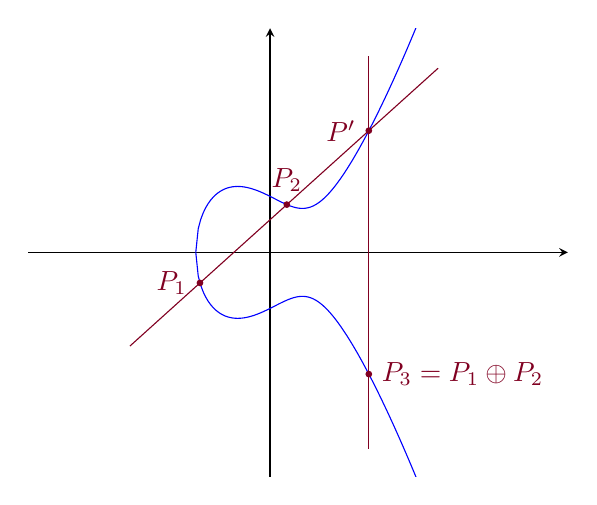
\begin{tikzpicture}
    \begin{axis}[
      xmin = -2, xmax = 3, ymin = -4, ymax = 4,
      axis equal,
      ticks = none,
      axis lines = middle,
      ]
      \addplot[domain=-1.32471796:3, blue, samples=100] {sqrt(x^3-x+1)};
      \addplot[domain=-1.32471796:3, blue, samples=100] {-sqrt(x^3-x+1)};
      \node[circle, burgundy, draw, fill, inner sep=0pt, minimum size=2pt, label={left:\textcolor{burgundy}{$P_1$}}] (P1) at (axis cs:-1.25,-0.54486) {};
      \node[circle, burgundy, draw, fill, inner sep=0pt, minimum size=2pt, label={above:\textcolor{burgundy}{$P_2$}}] (P2) at (axis cs:0.3,0.85264) {};
      \node[circle, burgundy, draw, fill, inner sep=0pt, minimum size=2pt, label={left:\textcolor{burgundy}{$P'$}}] (P3) at (axis cs:1.763, 2.17180) {};
      \addplot[domain=-2.5:3, burgundy] {0.90161*x+0.58216};
      \addplot[burgundy, mark=none] coordinates {(1.763, -3.5) (1.763, 3.5)};
      \node[circle, burgundy, draw, fill, inner sep=0pt, minimum size=2pt, label={right:\textcolor{burgundy}{$P_3 = P_1 \oplus P_2$}}] (P4) at (axis cs:1.763, -2.17180) {};
    \end{axis}
  \end{tikzpicture}
\end{figure}
and put $P_i = (x_i, y_i)$, $P'=(x',y')$.

Now $\ominus P_1 = (x_1, -(a_1x_1+a_3)-y_1)$, just by setting $y = -y_1$ in $(\ast)$.

The line through $P_1, P_2$ has equation say $y = \lambda x + \nu$. Substituting into $(\ast)$ and looking at the coefficient of $x^2$, we get:
\[\lambda^2 + a_1 \lambda - a_2 = x_1 + x_2 + x'\]
Since $x_3 = x'$, we have:
\begin{align*}
   x_3 &= \lambda^2+a_1\lambda-a_2-x_1-x_2\\
   y_3 &= -(a_1 x' + a_3) - y'\\
   &= -(\lambda+a_1)x_3 - \nu - a_3
\end{align*}
It remains to find $\lambda$ and $\nu$. There are 3 cases:
\begin{enumerate}
  \item $x_1=x_2, P_1 \neq P_2$.

  Then $P_1 \oplus P_2 = O_E$.

  \item $x_1 \neq x_2$.

  \[\lambda = \frac{y_2-y_1}{x_2-x_1},\;\; \nu = y_1-\lambda x_1 = \frac{y_1x_2-y_2x_1}{x_2-x_1}\]

  \item $P_1 = P_2$.

  Here we have to compute the equation of the tangent line etc. The solutions are:
  \[ \lambda=\frac{3x_1^2+2a_2x_1+a_4-a_1y_1}{2y_1+a_1x_1+a_3},\;\;\nu = \frac{-x_1^3+a_4x_1+2a_6-a_3y_1}{2y_1+a_1x_1+a_3}\]
\end{enumerate}

\begin{corollary}
  $E(K)$ is an abelian group.
\end{corollary}
\begin{proof}
  It is a subgroup of $E$ ($=E(\bar{K})$).

  \begin{itemize}[leftmargin=2cm]
    \item[Identity:] $O_E \in E(K)$ by definition.
    \item[Closure:] See formulae above.
    \item[Inverses:] See formulae above.
    \item[Associativity:] Inherited from $E(\bar{K})$.
    \item[Commutativity:] Inherited from $E(\bar{K})$.
  \end{itemize}
\end{proof}

If there is no ambiguity (i.e. we are not also adding numbers at the same time), the circles will be dropped from the group operation.
\begin{theorem}
  Elliptic curves are group varieties.

  i.e., $[-1]:E \to E; P\mapsto -P$ and $+:E\times E \to E; (P,Q)\mapsto P+Q$ are morphisms of algebraic varieties.
\end{theorem}
\begin{proof}
  The above formulae show that $[-1]$ and $+$ are rational maps. We know immediately that $[-1]$ is a morphism, as it is a rational map from a smooth curve to a projective variety.

  The formulae also show that $+$ is regular on the set
  \[ U = \{(P,Q) \in E \times E \mid P, Q, P+Q, P-Q \neq O_E\}\]
  For $P \in E$, let $\tau_P:E \to E; X \mapsto P+X$ be the ``translation by $P$" map.

  Then $\tau_P$ is a rational map from a smooth curve to a projective variety, so is a morphism.

  We factor $+$ as:
  \[ E\times E\xrightarrow[\tau_{-A}\times \tau_{-B}]{}E\times E \xrightarrow[\tau_{A+B}]{} E \xrightarrow[\tau_{A+B}]{} E\]

  Now $+$ is regular on $(\tau_A \times \tau_B)(U)$ for all $A, B \in E$, and so $+$ is regular on $E \times E$.
\end{proof}

\underline{\textbf{Definition.}} For any $n \in \Z_{>0}$, let $[n]: E \to E; P \mapsto P+\ldots+P$, $n$ times, and $[-n] = [-1]\circ [n]$, $[0]:P \mapsto O_E$ (i.e., the standard way of turning an abelian group into $\Z$ module).

\underline{\textbf{Definition.}} The \emph{n-torsion} subgroup of $E$ is $E[n] = \ker([n]:E\to E)$.

\begin{lemma}
  If $\charr(K) \neq 2$, and $E : y^2 = (x-e_1)(x-e_2)(x-e_3)$.

  Then $E[2] = (0, (e_1, 0), (e_2, 0), (e_3 0)) \cong (\Z/2\Z)^2$.
\end{lemma}
\begin{proof}
  Let $P = (x, y) \in E$. Then $[2]P = 0 \iff P = -P \iff (x, y) = (x, -y) \iff y = 0$.
\end{proof}

\subsection{Elliptic Curves over $\C$}
Let $\Lambda = \{a\omega_1 + b\omega_2 : a, b \in \Z\}$, where $\omega_1, \omega_2$ form a basis for $\C$ over $\R$.

Then the meromorphic functions on the Riemann surface (or lattice) $\C/\Lambda$ are the same as the $\Lambda$-invariant meromorphic functions on $\C$ (i.e. $f(z) = f(z+\lambda)$ for $\lambda \in \Lambda$).

This set of functions is a field, and is generated by $\wp(z)$ and $\wp'(z)$, where:
\begin{align*}
  \wp(z) = \frac{1}{z^2} + \sum_{0 \neq \lambda\in\Lambda} \left(\frac{1}{(z-\lambda)^2} - \frac{1}{\lambda^2}\right)
\end{align*}
They satisfy $\wp'(z)^2 = 4\wp(z)^3-g_2\wp(z)-g_3$, for some $g_1, g_3 \in \C$ depending on $\lambda$. We call $\wp$ the \emph{Weierstrass p-function}.

One can show that $\C/\Lambda \cong E(\C)$, where $E$ is the elliptic curve $y^2=4x^3-g_2x-g_3$. This is an isomorphism, not only of Riemann surfaces, but moreover of groups

\begin{theorem}[Uniformisation Theorem]
  Every elliptic curve over $\C$ arises in this way.
\end{theorem}

Thus, for elliptic curves $E/\C$, we have:
\begin{enumerate}[label=\protect\circled{\arabic*}]
  \item $E[n] \cong (\Z/n\Z)^2$
  \item $\deg[n] = n^2$
\end{enumerate}
We will show that \circled{2} holds over any field $K$, and \circled{1} holds if $\charr K \nmid n$.

\underline{Summary of Results} (N.B. the isomorphisms in 1, 2, 4 respect the relevant topologies)
\begin{enumerate}
  \item $K = \C$\hspace{2cm}$E(\C) \cong \C/\Lambda \cong \R/\Z\times \R/\Z$
  \item $K = \R$\hspace{2cm}$E(\R) \cong \begin{cases} \Z/2\Z \times \R/\Z & \Delta > 0 \\ \R/\Z & \Delta < 0\end{cases}$
  \item $K = \F_q$\hspace{1.9cm}$|\#E(\F_q) - (q+1)|\leq 2\sqrt{q}$
  \item $[K:\Q_p]<\infty$\hspace{1cm}$E(K)$ has a subgroup of finite index isomorphic to $(\O_K, +)$
  \item $[K:\Q]<\infty$\hspace{1.15cm}$E(K)$ is a finitely generated abelian group.
\end{enumerate}

\section{Isogenies}
Let $E_1, E_2$ be elliptic curves.

\textbf{Definition.} An \emph{isogeny} $\phi:E_1 \to E_2$ is a non-constant morphism taking $O_{E_1}$ to $O_{E_2}$, and we say $E_1$ and $E_2$ are \emph{isogenous} if there is an isogeny $E_1 \to E_2$.

\textbf{Definition.} $\Hom(E_1, E_2) = \{\text{isogenies } E_1 \to E_2\}\cup\{0\}$. This is a group under $(\phi+\psi)(P) = \phi(P)+\psi(P)$.

If $E_1 \xrightarrow{\phi} E_2 \xrightarrow{\psi} E_3$ are isogenies, then $\psi\phi$ is an isogeny. The tower law tells us that $\deg(\psi\phi) = \deg(\phi)\deg(\psi)$.

\begin{lemma}
  If $0 \neq n \in \Z$, then $[n] : E \to E$ is an isogeny.
\end{lemma}
\begin{proof}
  Theorem \textbf{4.4} tells us that $[n]$ is a morphism. We must show that $[n]\neq 0$.

  Assume $\charr K \neq 2$, then we can use Lemma \textbf{4.5}. If $n=2$, then $\#E[2] = 4$, and so $[2] \neq 0$.

  If $n$ is odd, then there is $0\neq T \in E[2]$. Then $nT = T \neq 0$, so $[n]$ is not the zero map.

  Now $[m][n] = [m]\circ[n]$, and any $n = 2^k m$ for $m$ odd, so $[n]$ is not the zero map for any $n \neq 0$.

  If $\charr K =2$, then replace \textbf{4.5} with a lemma computing $E[3]$.
\end{proof}
\textbf{Corollary.} \textit{$\Hom(E_1, E_2)$ is torsion-free as a $\Z$-module.}
\begin{lemma}
  Let $\phi:E_1 \to E_2$ be an isogeny. Then $\phi(P+Q) = \phi(P) + \phi(Q)$ for all $P, Q \in E_1$.
\end{lemma}
\begin{proof}[Sketch proof.]
  $\phi$ induces a map $\phi_\ast : \Div^0(E_1) \to \Div^0(E_2)$ given by $\sum\limits_{P\in E_1}n_p P \mapsto \sum\limits_{P \in E_1}n_p \phi(P)$.

  Recall that, via a pullback, $\phi^\ast : K(E_2) \injection K(E_1)$.

  If $f \in K(E_1)^\ast$, then $\phi_\ast(\div f)=\div(N_{K(E_1)/K(E_2)}f)$ - this is a fact that we'll take for granted.

  So $\phi_\ast$ takes principal divisors to principal divisors. Since $\phi(O_{E_1}) = O_{E_2}$, the following diagram commutes:
  \begin{tikzcd}
    E_1 \arrow{r}{\phi} \arrow{d}{\psi_1} & E_2 \arrow{d}{\psi_2}\\
    \Pic^0(E_1) \arrow{r}{\phi_\ast} & \Pic^0(E_2)
  \end{tikzcd}
  ,where $\psi_1:P \mapsto [(P) -(O_{E_1})], \psi_2:Q \mapsto [(Q)-(O_{E_2})]$.

  Since $\phi_\ast$ is a group homomorphism, $\phi$ is also a group homomorphism.
\end{proof}

\begin{lemma}
  Let $\phi:E_1\to E_2$ be an isogeny. Then there is a morphism $\xi$ making the following diagram commute:

  \begin{center}
    \begin{tikzcd}
      E_1 \arrow{r}{\phi} \arrow{d}{x_1} & E_2 \arrow{d}{x_2} \\
      \P^1 \arrow{r}{\xi} & \P^1
    \end{tikzcd}
  \end{center}

  where $x_i$ is the $x$-coordinate in a Weierstrass equation for $E_i$.

  Moreover, if $\xi(t) = \frac{r(t)}{s(t)}$ for $r, s \in K[t]$ coprime, then $\deg \phi = \deg \xi = \max(\deg r, \deg s)$.
\end{lemma}
\begin{proof}
  For $i = 1,2$, $K(E_i)/K(x_i)$ is a degree 2 extension, since the extension is given by adjoining $y_i$, which satisfies a quadratic (see the Weierstrass equation). Moreover, it is Galois, as $[-1]^\ast$ is a non-trivial automorphism of $K(E_i)$ fixing $K(x_i)$.

  Since $\phi$ is a group homomorphism, we have that $\phi(-P) = -\phi(P)$, i.e. $\phi \circ [-1] = [-1]\circ \phi$.

  If $f \in K(x_2)$, then $[-1]^\ast f = f$, and $[-1]^\ast (\phi^\ast f) = \phi^\ast ([-1]^\ast f) = \phi^\ast f$. Hence $\phi^\ast f$ is fixed by $[-1]$, so is in $K(x_1)$, and $K(x_2) \leq K(x_1)$.

  Taking $f = x_2$, then $\phi^\ast x_2 \in K(x_1)$, say $\xi(x_1)$ for some rational function $\xi$. Then $\xi$ is as required.

  Since $[K(E_1):K(x_1)] = [K(E_2):K(x_2)] = 2$, we have the following diagram of field extensions:
  \begin{center}
    \begin{tikzcd}
      & K(E_1) \arrow[dash, swap]{dl}{2} \arrow[dash]{dr}{\deg\phi} & \\
      K(x_1) \arrow[dash, swap]{dr}{\deg\xi} & & K(x_2) \arrow[dash]{dl}{2}\\
      & K(x_2) &
    \end{tikzcd}
  \end{center}
  Using the tower law, $\deg \phi = \deg \xi$. Now, $K(x_2) \injection K(x_1)$ via $x_2 \mapsto \xi(x_1) = \frac{r(x_1)}{s(x_2)}$ for $r, s \in K[t]$ coprime.

  The minimal polynomial of $x_1$ over $K(x_2)$ is $f(t) = r(t)-s(t)x_2 \in K(x_2)[t]$ - this is clearly a polynomial for $x_1$, but we need to check it's irreducible.

  $f$ is irreducible in $K[t][x_2] = K[x_2][t]$ as it is of degree 1 in $x_2$, so one of the factors must be constant in $x_2$, so divide both $r$ and $s$ which are coprime. Then we can use Gauss's lemma, and it is irreducible in $K(x_2)[t]$.

  Hence $\deg \phi = \deg \xi = [K(x_1):K(x_2)] = \deg (r(t)-s(t)x_2) = \max(\deg r, \deg s)$.
\end{proof}

\begin{lemma}
  $\deg[2] = 4$
\end{lemma}
\begin{proof}
  Assume $\charr K \neq 2, 3$. Then $E: y^2=x^3+ax+b=f(x)$.

  If $P = (x,y)$, then $x(2P) = \left(\frac{3x^2+a}{2y}\right)^2-2x = \frac{(3x^2+a)^2-8xf(x)}{4f(x)} = \frac{x^4+\ldots}{4f(x)}$.

  The numerator and denominator are coprime - suppose there was a common factor. Then $\exists \theta \in \bar{K}$ with $f(\theta) = (3\theta^2+a)^2 = f'(\theta) = 0$, and so $f$ has a multiple root. But $E$ is an elliptic curve so $f$ doesn't have multiple roots.

  Hence $\deg [2] = \max(\deg x^4+\ldots, \deg 4f(x)) = \max(4, 3) = 4$.
\end{proof}
\end{document}
